\section{Introducción}

\subsection{1.1 Motivación y Alcance}

Resulta particularmente llamativo observar cómo la construcción de infraestructuras espaciales de gran escala ha pasado de ser una aspiración conceptual a una necesidad operativa impostergable. Aunque los enfoques terrestres de integración previa han servido durante décadas, imponen restricciones severas de masa y volumen que los lanzadores actuales no pueden superar de manera económica. 

En este contexto, el ensamblaje robótico in-orbit emerge como alternativa estratégica. Revisiones exhaustivas recientes clasifican las tecnologías de ensamblaje y servicing en órbita, destacando sus ventajas para la creación de estructuras modulares de gran envergadura en comparación con métodos de ensamblaje exclusivamente terrestre \cite{Wang2025_OASR}. Particularmente relevante resulta la misión OSAM-1 de NASA, diseñada para demostrar capacidades de servicing, ensamblaje y manufactura en órbita, incluyendo operaciones de reabastecimiento robótico. Sus objetivos y las lecciones preliminares sobre gestión de riesgos en entornos impredecibles subrayan el potencial real de estos sistemas, aunque también revelan brechas persistentes en autonomía y eficiencia operativa \cite{NASA_OSAM1_2023}.

Uno de los desafíos persistentes que surge al analizar misiones de exploración profunda —hacia la Luna, Marte o asteroides— radica en la imposibilidad práctica de lanzar sistemas completamente ensamblados. El ensamblaje in-orbit no solo mitiga estos riesgos logísticos, sino que abre la puerta a arquitecturas escalables y reparables. No obstante, cabe matizar que la eficiencia actual de estas operaciones todavía dista de los estándares requeridos para misiones de larga duración, donde cada minuto adicional de actividad robótica impacta directamente en el consumo energético y la exposición a perturbaciones orbitales. El alcance de este trabajo se centra precisamente en optimizar dicha eficiencia mientras se reducen riesgos asociados a manipulación en microgravedad y coordinación multi-componente.

\subsection{1.2 Contribuciones Principales}

Lejos de ser un asunto resuelto, la literatura especializada tiende a subrayar limitaciones importantes en los manipuladores robóticos actuales para on-orbit servicing. Encuestas comprehensivas revelan avances notables en estimación de estado y técnicas de control basadas en machine learning, si bien la precisión y robustez en escenarios reales siguen representando un cuello de botella significativo \cite{Alizadeh2024_Survey}.

Las contribuciones principales de este artículo responden directamente a esas brechas. En primer lugar, se propone un framework híbrido de planificación y control que integra gemelos digitales para predicción en tiempo real de comportamientos estructurales durante el ensamblaje. En segundo lugar, se introducen métricas cuantitativas específicas de eficiencia orbital que combinan tiempo de montaje, consumo energético y probabilidad de fallo, permitiendo comparaciones sistemáticas más allá de enfoques cualitativos predominantes. Finalmente, se evalúa la reducción de riesgos en escenarios representativos de exploración profunda, demostrando mejoras mensurables frente a configuraciones mono-robot tradicionales.

Estas aportaciones no pretenden resolver todos los problemas del campo, pero sí avanzar de forma concreta hacia sistemas más autónomos y confiables.

\subsection{1.3 Organización del Documento}

El resto del artículo se estructura de manera que facilite la comprensión progresiva de la propuesta. La Sección 2 revisa el estado del arte y antecedentes relevantes. La Sección 3 detalla la metodología propuesta, incluyendo arquitectura del sistema, algoritmos de planificación y el rol del gemelo digital. Posteriormente, la Sección 4 describe la implementación y entorno de simulación, mientras que la Sección 5 presenta los resultados cuantitativos y análisis de sensibilidad. La Sección 6 discute implicaciones, limitaciones y comparaciones con trabajos previos. Finalmente, la Sección 7 recoge conclusiones principales junto con líneas de investigación futura.

\begin{figure}[h]
\centering
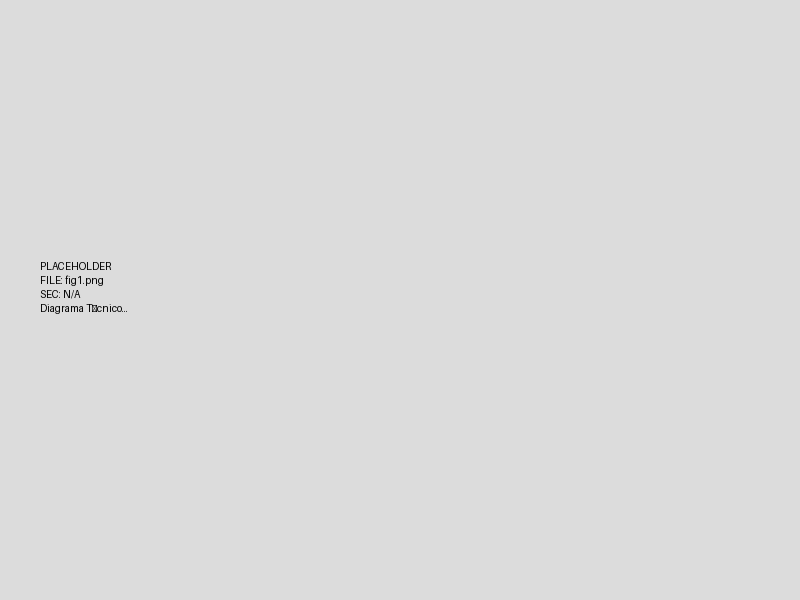
\includegraphics[width=\linewidth]{fig1.png}
\caption{Evolución cronológica de misiones clave de On-Orbit Servicing (OOS) y Assembly (OIRA), destacando hitos tecnológicos desde ETS-VII hasta proyectos actuales como OSAM-1.}
\label{fig:evolucion_misiones}
\end{figure}

\begin{table}[h]
\centering
\caption{Comparación de enfoques de ensamblaje orbital versus terrestre}
\label{tab:comparacion_enfoques}
\begin{tabular}{lcc}
\hline
\textbf{Criterio} & \textbf{Ensamblaje Terrestre} & \textbf{Ensamblaje In-Orbit} \\
\hline
Limitación de tamaño & Alta & Baja \\
Flexibilidad de reparación & Muy baja & Alta \\
Costo por kg en órbita & Elevado & Potencialmente menor \\
Riesgo durante lanzamiento & Alto & Reducido \\
Complejidad operativa & Media & Alta \\
\hline
\end{tabular}
\end{table}